\documentclass[tikz,border=2pt]{standalone}
\usepackage{fontspec}
\setmainfont{texgyreheros}[Extension=.otf,UprightFont=*-regular,BoldFont=*-bold,ItalicFont=*-italic]
\renewcommand{\familydefault}{\rmdefault}
\usepackage{amsmath}
\usetikzlibrary{arrows.meta,calc,positioning}
\begin{document}
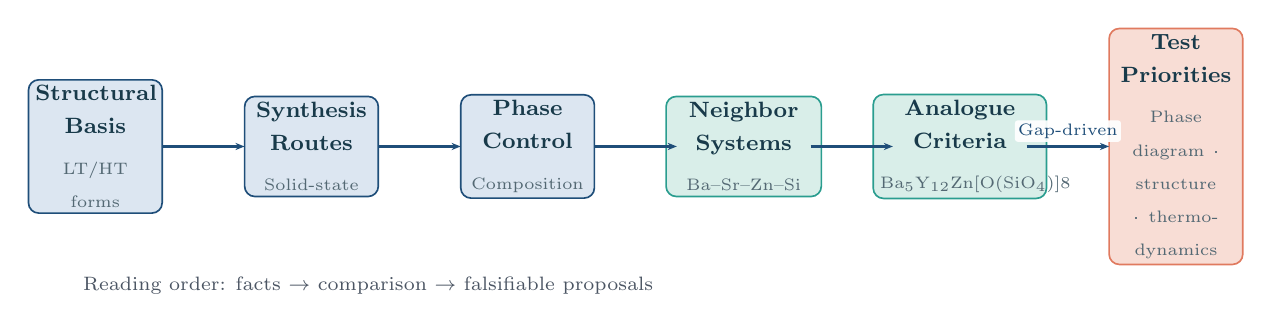
\begin{tikzpicture}[x=1pt,y=1pt, every node/.style={inner sep=0pt}]
\definecolor{nf}{HTML}{DCE6F1}\definecolor{ns}{HTML}{1f4e79}
\definecolor{lc}{HTML}{183A4A}\definecolor{sc}{HTML}{536873}
\node[draw=ns, fill=nf, line width=0.60pt, rounded corners=3.7pt, minimum width=48.3pt, minimum height=33.5pt, text width=43.3pt, align=center, inner sep=2pt, anchor=center, text opacity=0] at (31.61pt,132.02pt) {\hyphenpenalty=9000\exhyphenpenalty=9000\relax {\bfseries\fontsize{8.5}{10.1}\selectfont\color{lc}Structural Basis}\\[2.6pt]{\fontsize{6.1}{7.4}\selectfont\color{sc}LT/HT forms}};
\definecolor{nf}{HTML}{DCE6F1}\definecolor{ns}{HTML}{1f4e79}
\definecolor{lc}{HTML}{183A4A}\definecolor{sc}{HTML}{536873}
\node[draw=ns, fill=nf, line width=0.60pt, rounded corners=3.7pt, minimum width=48.3pt, minimum height=33.5pt, text width=43.3pt, align=center, inner sep=2pt, anchor=center, text opacity=0] at (109.71pt,132.02pt) {\hyphenpenalty=9000\exhyphenpenalty=9000\relax {\bfseries\fontsize{8.5}{10.1}\selectfont\color{lc}Synthesis Routes}\\[2.6pt]{\fontsize{6.1}{7.4}\selectfont\color{sc}Solid-state}};
\definecolor{nf}{HTML}{DCE6F1}\definecolor{ns}{HTML}{1f4e79}
\definecolor{lc}{HTML}{183A4A}\definecolor{sc}{HTML}{536873}
\node[draw=ns, fill=nf, line width=0.60pt, rounded corners=3.7pt, minimum width=48.3pt, minimum height=33.5pt, text width=43.3pt, align=center, inner sep=2pt, anchor=center, text opacity=0] at (187.80pt,132.02pt) {\hyphenpenalty=9000\exhyphenpenalty=9000\relax {\bfseries\fontsize{8.5}{10.1}\selectfont\color{lc}Phase Control}\\[2.6pt]{\fontsize{6.1}{7.4}\selectfont\color{sc}Composition}};
\definecolor{nf}{HTML}{D9EEE9}\definecolor{ns}{HTML}{2a9d8f}
\definecolor{lc}{HTML}{183A4A}\definecolor{sc}{HTML}{536873}
\node[draw=ns, fill=nf, line width=0.60pt, rounded corners=3.7pt, minimum width=56.1pt, minimum height=33.5pt, text width=51.1pt, align=center, inner sep=2pt, anchor=center, text opacity=0] at (265.90pt,132.02pt) {\hyphenpenalty=9000\exhyphenpenalty=9000\relax {\bfseries\fontsize{8.5}{10.1}\selectfont\color{lc}Neighbor Systems}\\[2.6pt]{\fontsize{6.1}{7.4}\selectfont\color{sc}Ba--Sr--Zn--Si}};
\definecolor{nf}{HTML}{D9EEE9}\definecolor{ns}{HTML}{2a9d8f}
\definecolor{lc}{HTML}{183A4A}\definecolor{sc}{HTML}{536873}
\node[draw=ns, fill=nf, line width=0.60pt, rounded corners=3.7pt, minimum width=62.6pt, minimum height=33.5pt, text width=57.6pt, align=center, inner sep=2pt, anchor=center, text opacity=0] at (344.00pt,132.02pt) {\hyphenpenalty=9000\exhyphenpenalty=9000\relax {\bfseries\fontsize{8.2}{9.7}\selectfont\color{lc}Analogue Criteria}\\[2.5pt]{\fontsize{5.9}{7.1}\selectfont\color{sc}Ba$_{5}$Y$_{12}$Zn[O(SiO$_{4}$)]8}};
\definecolor{nf}{HTML}{F8DDD5}\definecolor{ns}{HTML}{e07a5f}
\definecolor{lc}{HTML}{183A4A}\definecolor{sc}{HTML}{536873}
\node[draw=ns, fill=nf, line width=0.60pt, rounded corners=3.7pt, minimum width=48.3pt, minimum height=33.5pt, text width=43.3pt, align=center, inner sep=2pt, anchor=center, text opacity=0] at (422.09pt,132.02pt) {\hyphenpenalty=9000\exhyphenpenalty=9000\relax {\bfseries\fontsize{8.5}{10.1}\selectfont\color{lc}Test Priorities}\\[2.6pt]{\fontsize{6.1}{7.4}\selectfont\color{sc}Phase diagram · structure · thermodynamics}};
\definecolor{ec}{HTML}{1f4e79}
\draw[draw=ec, line width=1.12pt, -{Stealth[length=3.3pt,width=2.6pt]}, rounded corners=2.2pt] (55.78pt,132.02pt) -- (85.53pt,132.02pt);
\definecolor{ec}{HTML}{1f4e79}
\draw[draw=ec, line width=1.12pt, -{Stealth[length=3.3pt,width=2.6pt]}, rounded corners=2.2pt] (133.88pt,132.02pt) -- (163.63pt,132.02pt);
\definecolor{ec}{HTML}{1f4e79}
\draw[draw=ec, line width=1.12pt, -{Stealth[length=3.3pt,width=2.6pt]}, rounded corners=2.2pt] (211.98pt,132.02pt) -- (241.73pt,132.02pt);
\definecolor{ec}{HTML}{1f4e79}
\draw[draw=ec, line width=1.12pt, -{Stealth[length=3.3pt,width=2.6pt]}, rounded corners=2.2pt] (290.07pt,132.02pt) -- (319.82pt,132.02pt);
\definecolor{ec}{HTML}{1f4e79}
\draw[draw=ec, line width=1.12pt, -{Stealth[length=3.3pt,width=2.6pt]}, rounded corners=2.2pt] (368.17pt,132.02pt) -- (397.92pt,132.02pt);
\node[fill=white, fill opacity=0.92, text opacity=1, inner sep=1.2pt, rounded corners=1pt, font=\fontsize{5.6}{6.3}\selectfont, text=ec, anchor=south, align=center] at (383.05pt,133.51pt) {Gap-driven};
\definecolor{lc}{HTML}{183A4A}\definecolor{sc}{HTML}{536873}
\node[minimum width=48.3pt, minimum height=33.5pt, text width=43.3pt, align=center, inner sep=2pt, anchor=center] at (31.61pt,132.02pt) {\hyphenpenalty=9000\exhyphenpenalty=9000\relax {\bfseries\fontsize{8.5}{10.1}\selectfont\color{lc}Structural Basis}\\[2.6pt]{\fontsize{6.1}{7.4}\selectfont\color{sc}LT/HT forms}};
\definecolor{lc}{HTML}{183A4A}\definecolor{sc}{HTML}{536873}
\node[minimum width=48.3pt, minimum height=33.5pt, text width=43.3pt, align=center, inner sep=2pt, anchor=center] at (109.71pt,132.02pt) {\hyphenpenalty=9000\exhyphenpenalty=9000\relax {\bfseries\fontsize{8.5}{10.1}\selectfont\color{lc}Synthesis Routes}\\[2.6pt]{\fontsize{6.1}{7.4}\selectfont\color{sc}Solid-state}};
\definecolor{lc}{HTML}{183A4A}\definecolor{sc}{HTML}{536873}
\node[minimum width=48.3pt, minimum height=33.5pt, text width=43.3pt, align=center, inner sep=2pt, anchor=center] at (187.80pt,132.02pt) {\hyphenpenalty=9000\exhyphenpenalty=9000\relax {\bfseries\fontsize{8.5}{10.1}\selectfont\color{lc}Phase Control}\\[2.6pt]{\fontsize{6.1}{7.4}\selectfont\color{sc}Composition}};
\definecolor{lc}{HTML}{183A4A}\definecolor{sc}{HTML}{536873}
\node[minimum width=56.1pt, minimum height=33.5pt, text width=51.1pt, align=center, inner sep=2pt, anchor=center] at (265.90pt,132.02pt) {\hyphenpenalty=9000\exhyphenpenalty=9000\relax {\bfseries\fontsize{8.5}{10.1}\selectfont\color{lc}Neighbor Systems}\\[2.6pt]{\fontsize{6.1}{7.4}\selectfont\color{sc}Ba--Sr--Zn--Si}};
\definecolor{lc}{HTML}{183A4A}\definecolor{sc}{HTML}{536873}
\node[minimum width=62.6pt, minimum height=33.5pt, text width=57.6pt, align=center, inner sep=2pt, anchor=center] at (344.00pt,132.02pt) {\hyphenpenalty=9000\exhyphenpenalty=9000\relax {\bfseries\fontsize{8.2}{9.7}\selectfont\color{lc}Analogue Criteria}\\[2.5pt]{\fontsize{5.9}{7.1}\selectfont\color{sc}Ba$_{5}$Y$_{12}$Zn[O(SiO$_{4}$)]8}};
\definecolor{lc}{HTML}{183A4A}\definecolor{sc}{HTML}{536873}
\node[minimum width=48.3pt, minimum height=33.5pt, text width=43.3pt, align=center, inner sep=2pt, anchor=center] at (422.09pt,132.02pt) {\hyphenpenalty=9000\exhyphenpenalty=9000\relax {\bfseries\fontsize{8.5}{10.1}\selectfont\color{lc}Test Priorities}\\[2.6pt]{\fontsize{6.1}{7.4}\selectfont\color{sc}Phase diagram · structure · thermodynamics}};
\definecolor{tc}{HTML}{4b5563}
\node[anchor=center, font=\fontsize{7.2}{8.7}\selectfont, text=tc] at (130.16pt,81.82pt) {Reading order: facts $\rightarrow$ comparison $\rightarrow$ falsifiable proposals};
\end{tikzpicture}
\end{document}